
%\subsubsection{International Patent Classification code}
%In 1971, the Strasbourg Agreement established the International Patent Classification (IPC) under the World Intellectual Property Organization (WIPO), which divides technology into eight discrete Sections. The goal of this
%Agreement was to overcome the difficulties caused by using diverse national patent classification systems.~\citep{harris2010comparison}
%
%A patent is assigned to one or more of the 71,000 IPC codes that 
%indicate the related technical field or fields the patent covers. 
%These codes are arranged in a hierarchical, tree-like structure with 
%five distinct components. Fig. \ref{fig:ipcexample} illustrates the components of an IPC classification.
%
%The highest hierarchical level contains the eight sections of the IPC corresponding
%to very broad technical fields, labeled A through H. For example, Section C deals
%with``Chemistry and Metallurgy''. Sections are subdivided into classes. The eighth edition of the IPC contains 120
%classes. Class C07, for example, deals with ``Organic Chemistry''. Classes are further subdivided into more than 600 subclasses. Subclass C07C, for example, deals with ``Acyclic or Carbocyclic Compounds''. Subclasses are then further divided into main groups and subgroups. Main group symbols end with ``/00''. Ten percent of all IPC groups are main
%groups. For example, main group C07C 35/00 deals with ``Compounds having at
%least one hydroxy or O-metal group bound to a carbon atom of a ring other than
%a six-membered aromatic ring''. In some versions of the IPC, a series of numbers will follow the subgroup, reflecting
%the enactment date of the IPC version. `20060101' following the Subgroup
%indicates a date of January 1, 2006, which is the date that the eighth version of
%the IPC took effect. 
%%%%%%%%%%%%%%%%%%%%%%%%%%%%%%%%%%%%%%%%%%%%%%%%%%%%%%%%%%%%%%%%%%%%%%%%%%%%%%%%%%
%\begin{figure}[t!]
%   \centering
%   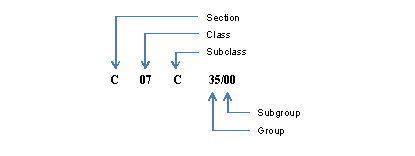
\includegraphics[width=0.70\textwidth,height=35mm]{figs/IPCexample.jpg}
%   \caption{An example illustrating the components of an International Patent Classification code.}   
%   \label{fig:ipcexample} 
%\end{figure}
%%%%%%%%%%%%%%%%%%%%%%%%%%%%%%%%%%%%%%%%%%%%%%%%%%%%%%%%%%%%%%%%%%%%%%%%%%%%%%%%%%
%\subsubsection{IPC Classification as a Filter}
As we mentioned in Section~\ref{sec:settings}, IPC codes (Section~\ref{StructureofPatents}) 
are assigned to patent queries to filter the search results by constraining them to have common IPC codes with the patent query.
In this section, we investigate the errors caused by classification code mismatch between topics (queries) and relevant documents for three different level of hierarchy. 
 
%\subsubsection{Applying 4-digit IPC code for filtering}
%\label{subsec: 4-digit}
\paragraph{Filter Type I: Three First Components of IPC Code}
\ \\
First, we examine the effect of filtering out the patents, which their three first symbols of IPC code, including section, class, and subclass (e.g., $\mathit{C07C}$ in Figure~\ref{fig:ipcexample}), do not match with the patent query. We have applied this filter to our baseline system. As a consequence, relevant patents, which do not share these three symbols of the IPC code with the patent query, are not retrieved by the system.   

Our experiments show that   
around 19\% of the not-retrieved relevant patents do not share any IPC code with the patent query, but the majority of them have main IPC code of the query, and about 21\% have, at least, one of the further IPC codes of the query (Figure~\ref{fig:ipcoverlap_a}). 
%%%%%%%%%%%%%%%%%%%%%%%%%%%%%%%%%%%%%%%%%%%%%%%%%%%%%%%%%%%%%%%%%%%%%%%%%%%%%%%%%
%\begin{figure}[t!]
%   \centering
%   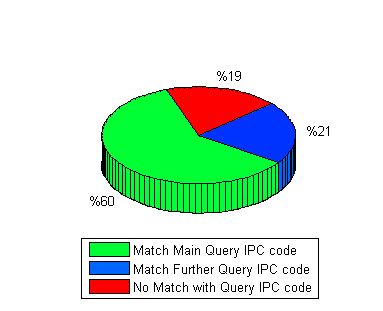
\includegraphics[width=0.60\textwidth,height=69mm]{figs/ipcOverlap-FNs.png}
%   \caption{Classification code overlap between the query and non-relevant retrieved patents (False Negative (FN) patents).}   
%   \label{fig:fnipcoverlap} 
%\end{figure}
%%%%%%%%%%%%%%%%%%%%%%%%%%%%%%%%%%%%%%%%%%%%%%%%%%%%%%%%%%%%%%%%%%%%%%%%%%%%%%%%%
%%%%%%%%%%%%%%%%%%%%%%%%%%%%%%%%%%%%%%%%%%%%%%%%%%%%%%%%%%%%%%
\begin{figure}[t!]
\begin{centering}
\subfigure[Not-retrieved relevant patents (False Negative (FN) patents)\label{fig:ipcoverlap_a}]{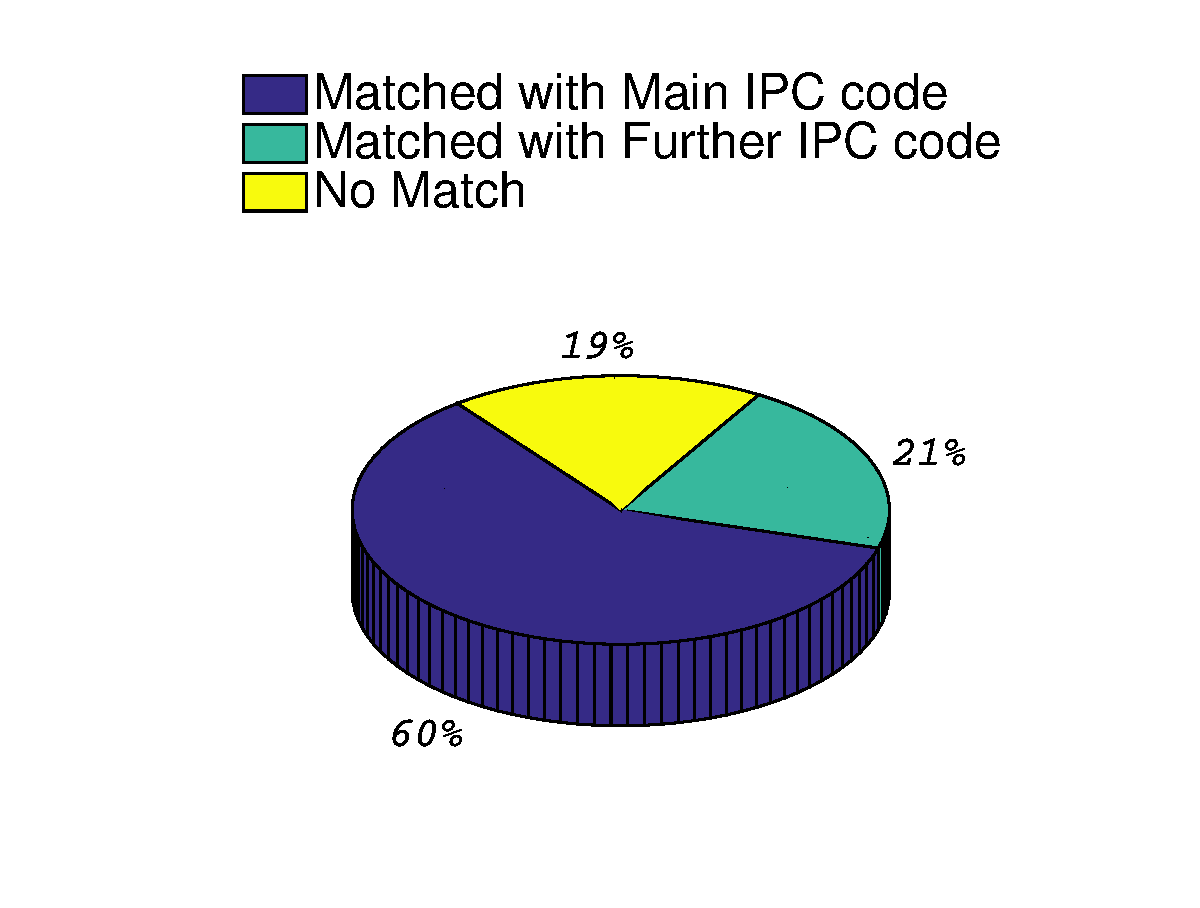
\includegraphics[width=6.5cm]{figs/ipcOverlap-FNs.eps}} 
\hspace*{0.5cm}  \subfigure[Retrieved relevant patents (True Positive (TP) patents)\label{fig:ipcoverlap_b}]{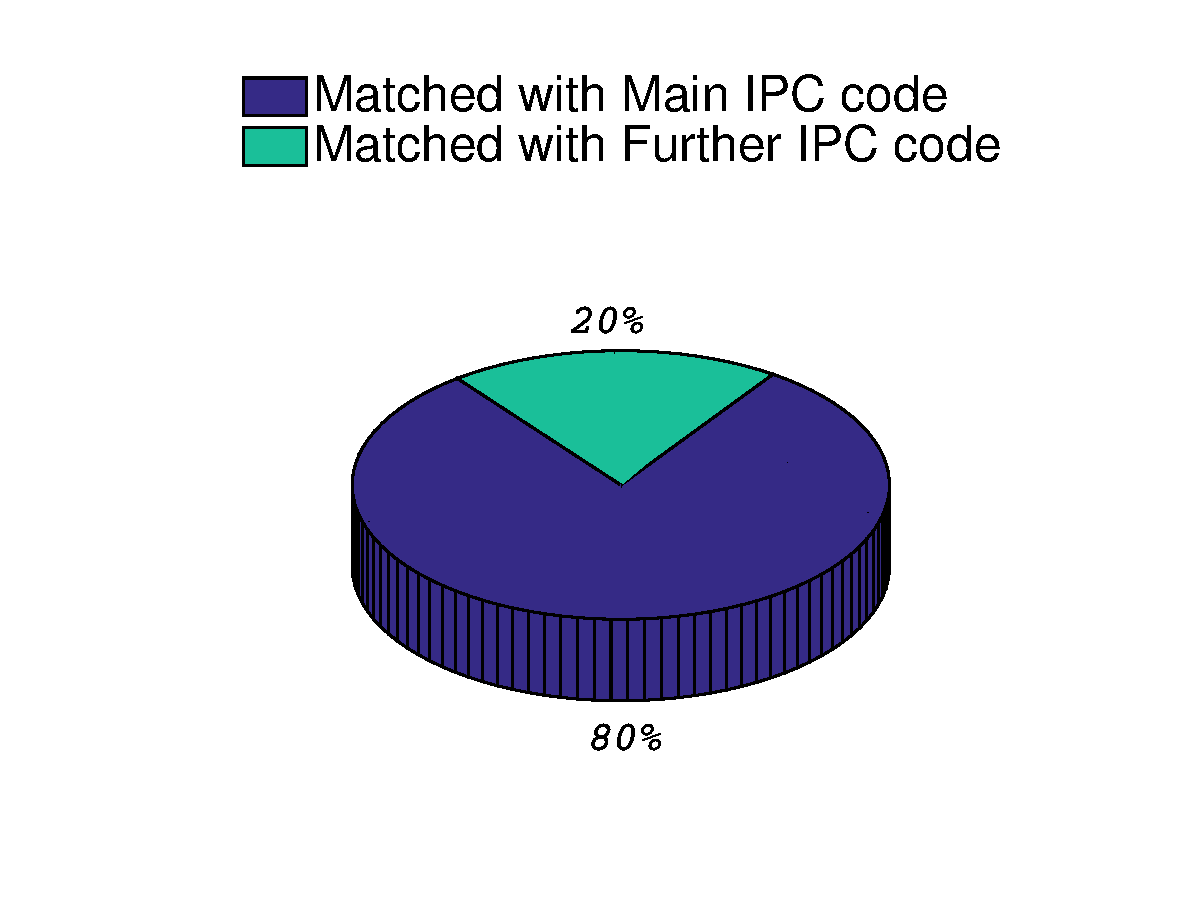
\includegraphics[width=6.5cm]{figs/ipcOverlap-TPs.eps}} 

\par\end{centering} 
\protect\caption{Classification code overlap between the query and non-relevant retrieved patents (False Negative (FN) patents).}
\label{fig:ipcoverlap}
\end{figure}
%%%%%%%%%%%%%%%%%%%%%%%%%%%%%%%%%%%%%%%%%%%%%%%%%%%%%%%%%%%%%%
We repeat the experiments for the true positive (TP) patents; as it has been shown in Figure \ref{fig:ipcoverlap_b}, 80\% of TP patents have an overlap with the main IPC code of the query and 20\% with, at least, one of the query further IPC codes. 
%So, we can conclude that 19\% of errors can be due to IPC filtering if we assume that they have enough term overlap with the query.  
%%%%%%%%%%%%%%%%%%%%%%%%%%%%%%%%%%%%%%%%%%%%%%%%%%%%%%%%%%%%%%%%%%%%%%%%%%%%%%%%%
%\begin{figure}[t!]
%   \centering
%   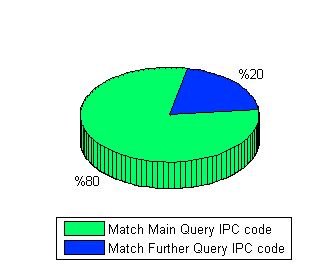
\includegraphics[width=0.55\textwidth,height=60mm]{figs/ipcOverlap-TPs.png}
%   \caption{Classification code overlap between the query and relevant retrieved patents (True Positive (TP) patents).}   
%   \label{fig:tpipcoverlap} 
%\end{figure}
%%%%%%%%%%%%%%%%%%%%%%%%%%%%%%%%%%%%%%%%%%%%%%%%%%%%%%%%%%%%%%%%%%%%%%%%%%%%%%%%%
Although we cannot retrieve around 19\% of relevant patents as a result of applying the IPC filter, we still keep using the filter in our experiments for the following two main reasons: 
\begin{enumerate}
\item CLEF-IP 2010 collection contains 2.6 million patent documents. If we do not use the IPC filter, it will take long time to compare each patent in the whole collection with the query. Nonetheless, if we apply the filter, this process will take faster because the matching process is done on only the portion of the collection, which shares an IPC code with the patent query not the whole collection. Since only less than 19\% of errors are due to a classification mismatch, we continue our analysis by keeping the filter on. The matching process is computationally much faster when we apply the IPC filter. In trade off between losing the percentage of the relevant patents and faster computation, we choose the efficient computation. The computational time is critical in patent prior art search because the query is the description of the the patent query, consisting of thousands of words.   
\item The precision in the top $k(=100)$ significantly drops, when we rank the whole collection versus only a subset of patents that have the same classification code with the patent query.  
\end{enumerate}

We conduct the following experiment to justify the first above-mentioned reason. First, we calculate the number of documents that should be processed during the ranking process per query after applying the filter. Then we plot the distribution of this number over all test topics.
%%%%%%%%%%%%%%%%%%%%%%%%%%%%%%%%%%%%%%%%%%%%%%%%%%%%%%%%%%%%%%%%%%%%%%%%%%%%%%%%%
\begin{figure}[t!]
   \centering
   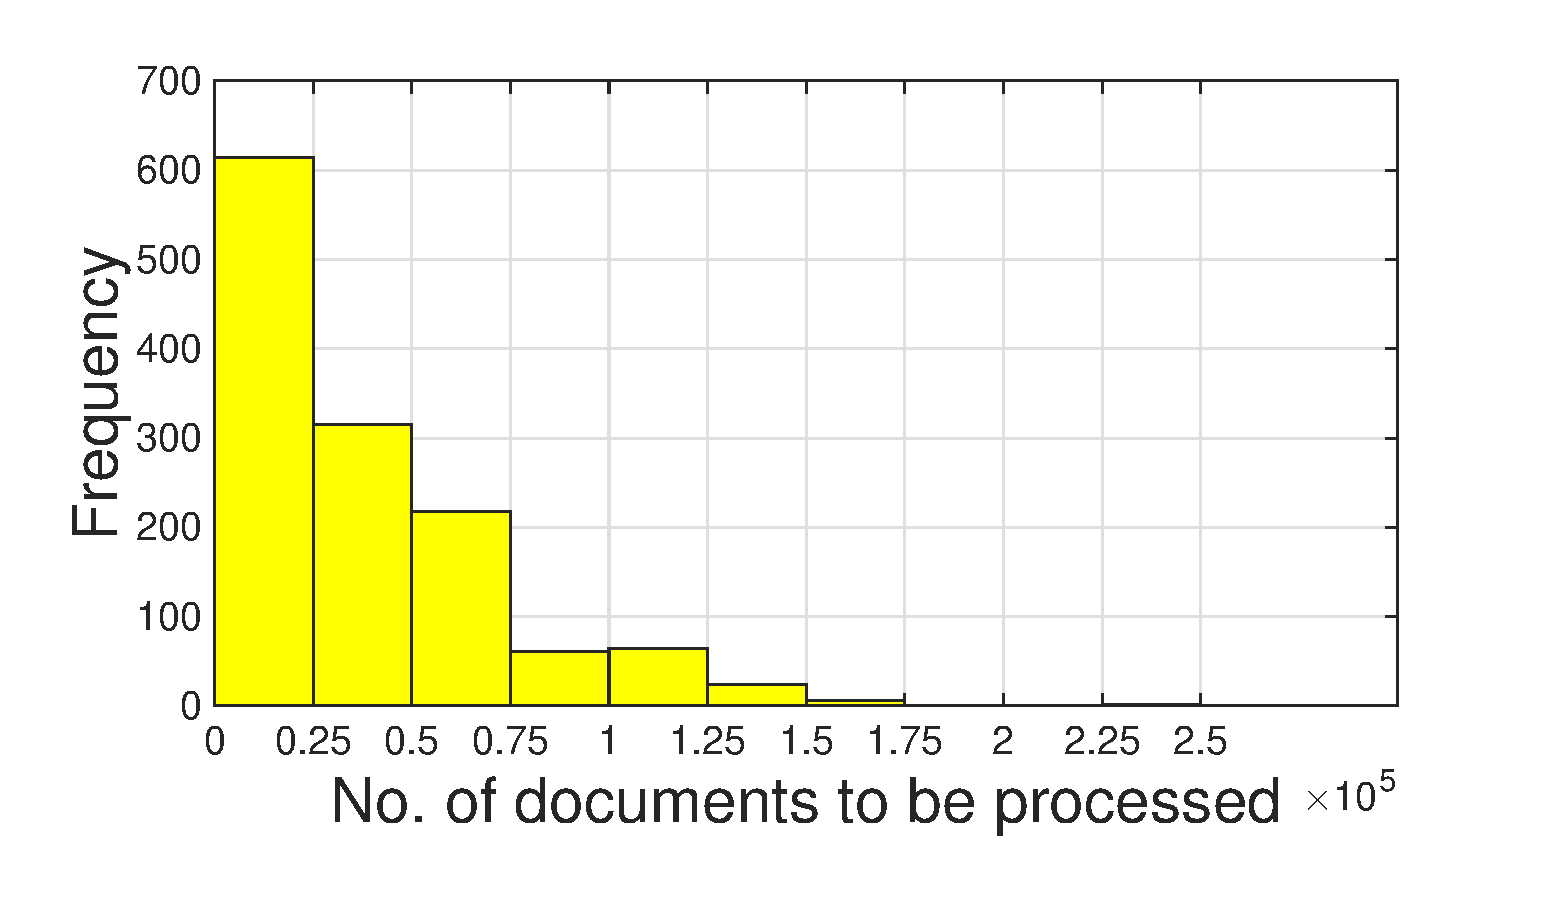
\includegraphics[width=0.70\textwidth,height=55mm]{figs/filter1}
   \caption{The distribution of the number of patents that should be ranked for each query over all test topics ($1,303$), after applying the IPC filter (filter type I).
On average, the matching process for each query is done over $ 36,254 $ documents instead of the whole collection (2.6 million documents), which dramatically reduces the computational time.}   
   \label{fig:ipcfilter-histo} 
\end{figure}
%%%%%%%%%%%%%%%%%%%%%%%%%%%%%%%%%%%%%%%%%%%%%%%%%%%%%%%%%%%%%%%%%%%%%%%%%%%%%%%%%
%\FloatBarrier 
%\noindent
Figure~\ref{fig:ipcfilter-histo} illustrates that the matching process should be only done over $25,000$ documents for the majority of queries. On average, this number is $ 36,254 $, which indicates that the system just needs to look into $ 36,254 $ documents per query on average instead of the entire collection that contains 2.6 million patent documents. Therefore, applying the IPC filter computationally saves us considerable amount of time.   

In trade off between losing 19\% of relevant patents and making the ranking process faster, we choose faster computation. In addition, we notice that the histogram falls down by increasing the number of documents that should be processed; this means that for the majority of queries the matching process is done over less number of patent documents.
%\vspace{-1cm}
%\subsubsection{Applying First two IPC code components for filtering}
%\label{subsec: Firsttwocomponents}
\paragraph{Filter Type II: Two First Components of IPC Code}
%\textbf{(B) Filter: First two components of the IPC code}
\ \\
We hypothesise that the errors will be reduced, if we broaden the filter by selecting two first components of the query IPC, namely, section, and class (e.g., C07). We repeat the experiments for filter type II.
The results have been illustrated in Figure~\ref{fig:ipc1stTwoElements}. Figure~\ref{fig:ipc1stTwoElements_a} shows that we can reduce the errors related to filtering from 19\% to 13\% by omitting the subclass component. However, the number of documents that should be ranked increases from $ 36,254 $ to $ 99,754 $ on average. As it can be seen in Figure~\ref{fig:ipc1stTwoElements_b}, the distribution of the number of documents that should be compared in matching process does not follow the falling trend as filtering with three first components. We conclude that this filter is not appropriate since we only reduce the error by 6\% whereas the average number of documents, which should be processed, triples.    
%%%%%%%%%%%%%%%%%%%%%%%%%%%%%%%%%%%%%%%%%%%%%%%%%%%%%%%%%%%%%%%%%%%%%%%%%%%%%%%%%
%\begin{figure}[t!]
%   \centering
%   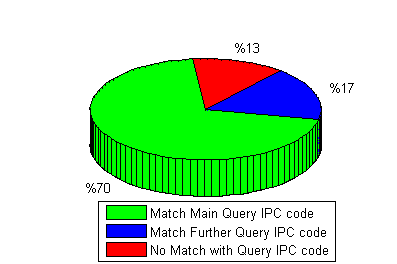
\includegraphics[width=0.55\textwidth,height=60mm]{figs/ipc1stTwoElements.png}
%   \caption{Filter: The first two components (Section and Class).}   
%   \label{fig:ipc1stTwoElements} 
%\end{figure}
%%%%%%%%%%%%%%%%%%%%%%%%%%%%%%%%%%%%%%%%%%%%%%%%%%%%%%%%%%%%%%%%%%%%%%%%%%%%%%%%%
%%%%%%%%%%%%%%%%%%%%%%%%%%%%%%%%%%%%%%%%%%%%%%%%%%%%%%%%%%%%%%
\begin{figure}[t!]
\begin{centering}
\subfigure[The portion of patents in the collection which are matched with the query IPC code. \label{fig:ipc1stTwoElements_a}]{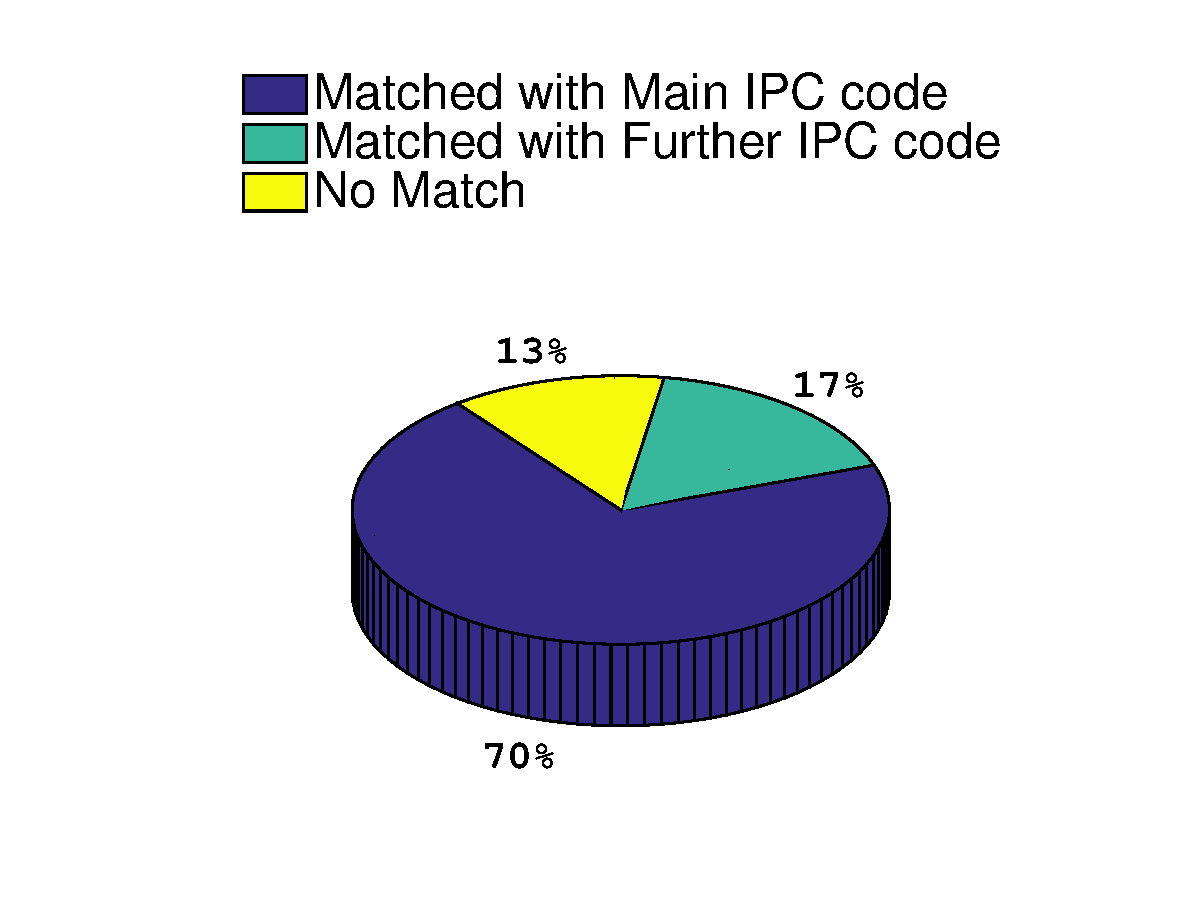
\includegraphics[width=7.5cm, height=6cm]{figs/filter2_pie}} 
\\[1ex]%
\subfigure[The distribution of the number of patents should be ranked for each query over all test queries ($1,303$).
In average, the matching process for each query is done over $ 99,754 $ documents instead of the whole collection (2.6 million documents), which dramatically reduce the computational time.\label{fig:ipc1stTwoElements_b}]{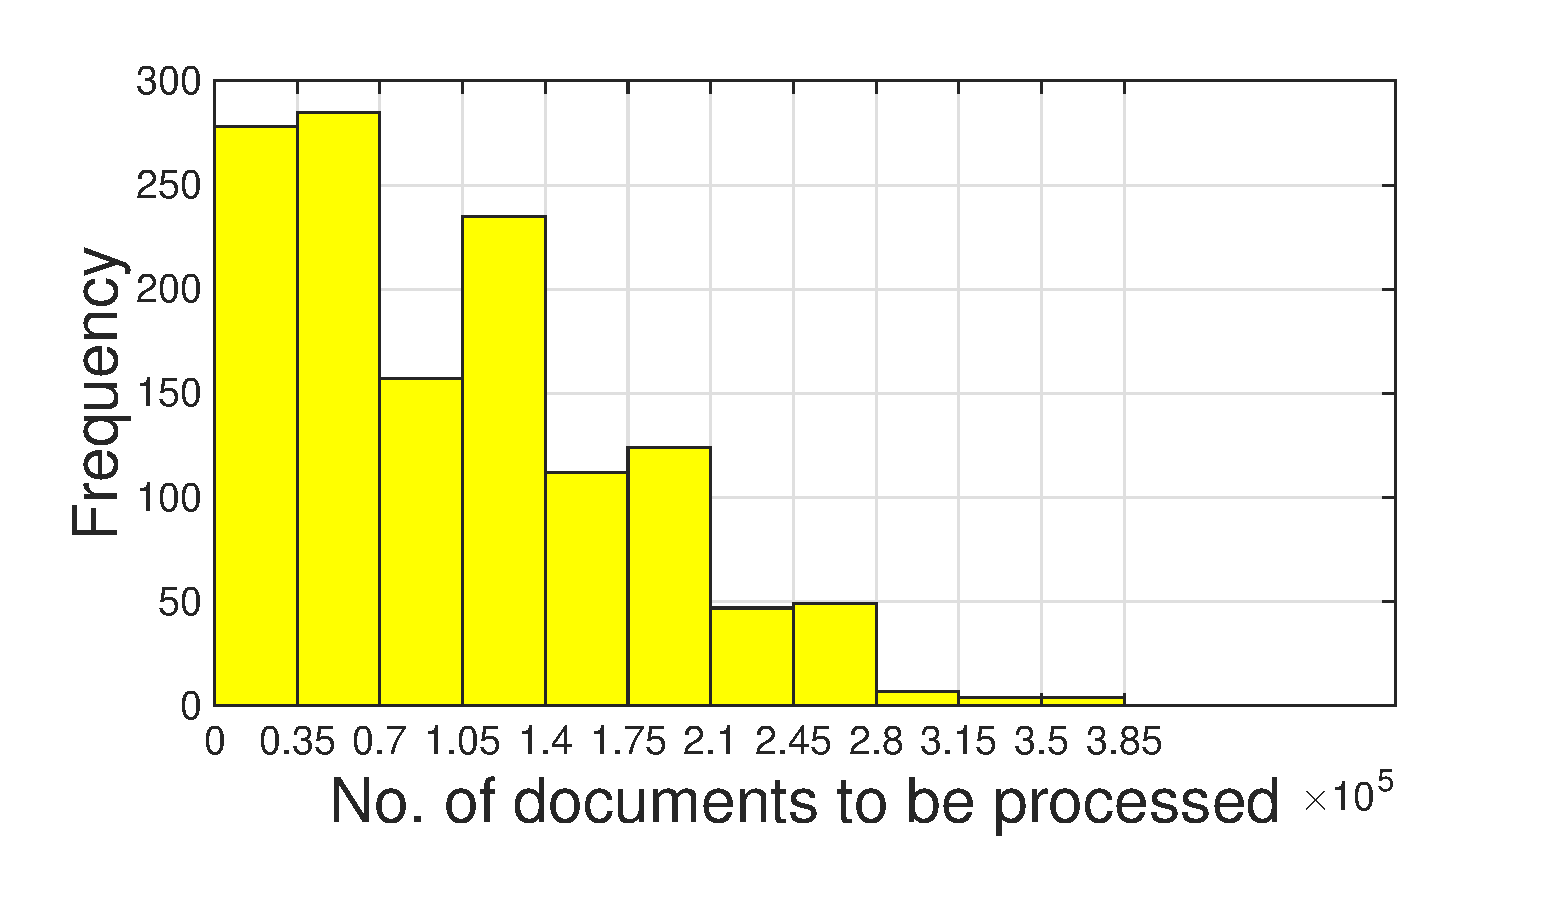
\includegraphics[width=9.5cm, height=6cm]{figs/filter2}} 

\par\end{centering} 
\protect\caption{Applying first two IPC code components (Section and Class) for filtering}
\label{fig:ipc1stTwoElements}
\end{figure}
%%%%%%%%%%%%%%%%%%%%%%%%%%%%%%%%%%%%%%%%%%%%%%%%%%%%%%%%%%%%%%
%\begin{figure}[htpb]
%\centering
%\begin{subfigure}[htpb]{.5\linewidth}
%\centering
%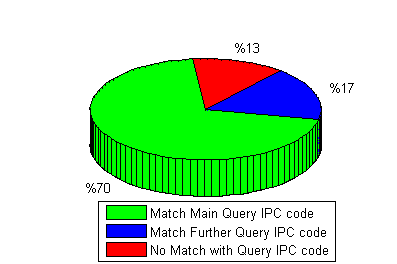
\includegraphics[width=1\textwidth,height=55mm]{figs/ipc1stTwoElements.png}
%\caption{Filter: The first two components (Section and Class)}
%\label{fig:ipc1stTwoElements}
%\end{subfigure}%\\[1ex]%
%\begin{subfigure}[htpb]{.5\linewidth}
%\centering
%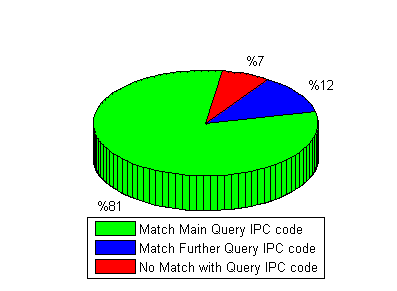
\includegraphics[width=1\textwidth,height=55mm]{figs/ipc1stElement.png}
%\caption{Filter: Only the first component (Section)}
%\label{fig:ipc1stElement}
%\end{subfigure}
%\caption{IPC classification overlap between the query and the FN patents after making the filter broader.}
%\label{fig:restrictedipc}
%\end{figure}
%\FloatBarrier
%%%%%%%%%%%%%%%%%%%%%%%%%%%%%%%%%%%%%%%%%%%%%%%%%%%%%%%%%%%%%%%%%%%%%%%%%%%%%%%%%
%\begin{figure}[t!]
%   \centering
%   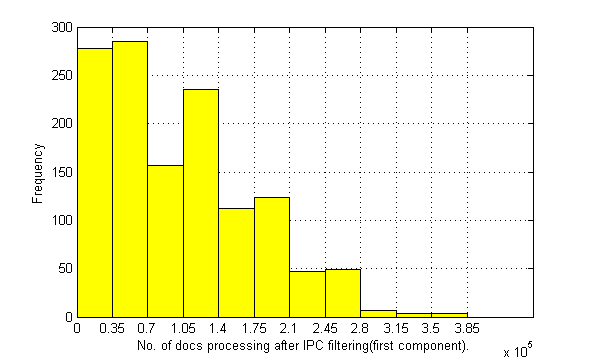
\includegraphics[width=0.70\textwidth,height=68mm]{figs/firstTwoIpcFilter-histo.png}
%   \caption{The distribution of the number of patents should be ranked for each query over all test queries (1303).
%In average, the matching process for each query is done over `$ 99754 $' documents instead of the whole collection (2.6 million documents) which reduce the computational time dramatically.}   
%   \label{fig:firstTwoIpcFilter-histo} 
%\end{figure}
%%%%%%%%%%%%%%%%%%%%%%%%%%%%%%%%%%%%%%%%%%%%%%%%%%%%%%%%%%%%%%%%%%%%%%%%%%%%%%%%%
%\FloatBarrier 
%\vspace{-5em}
%\noindent
%\subsubsection{Applying First two IPC code components for filtering}
%\label{subsec: Firsttwocomponents}
\paragraph{Filter Type III: First Component of IPC Code}
%\textbf{(C) Filter: First component of the IPC code}
\ \\
We can even make the filter more general by choosing only the first component, namely, section (e.g., C), corresponding to very general technical fields. 
%%%%%%%%%%%%%%%%%%%%%%%%%%%%%%%%%%%%%%%%%%%%%%%%%%%%%%%%%%%%%%
\begin{figure}[t!]
\begin{centering}
\subfigure[The portion of patents in the collection which are matched with the query IPC code. Filter: The first two components \label{fig:ipc1stElements_a}]{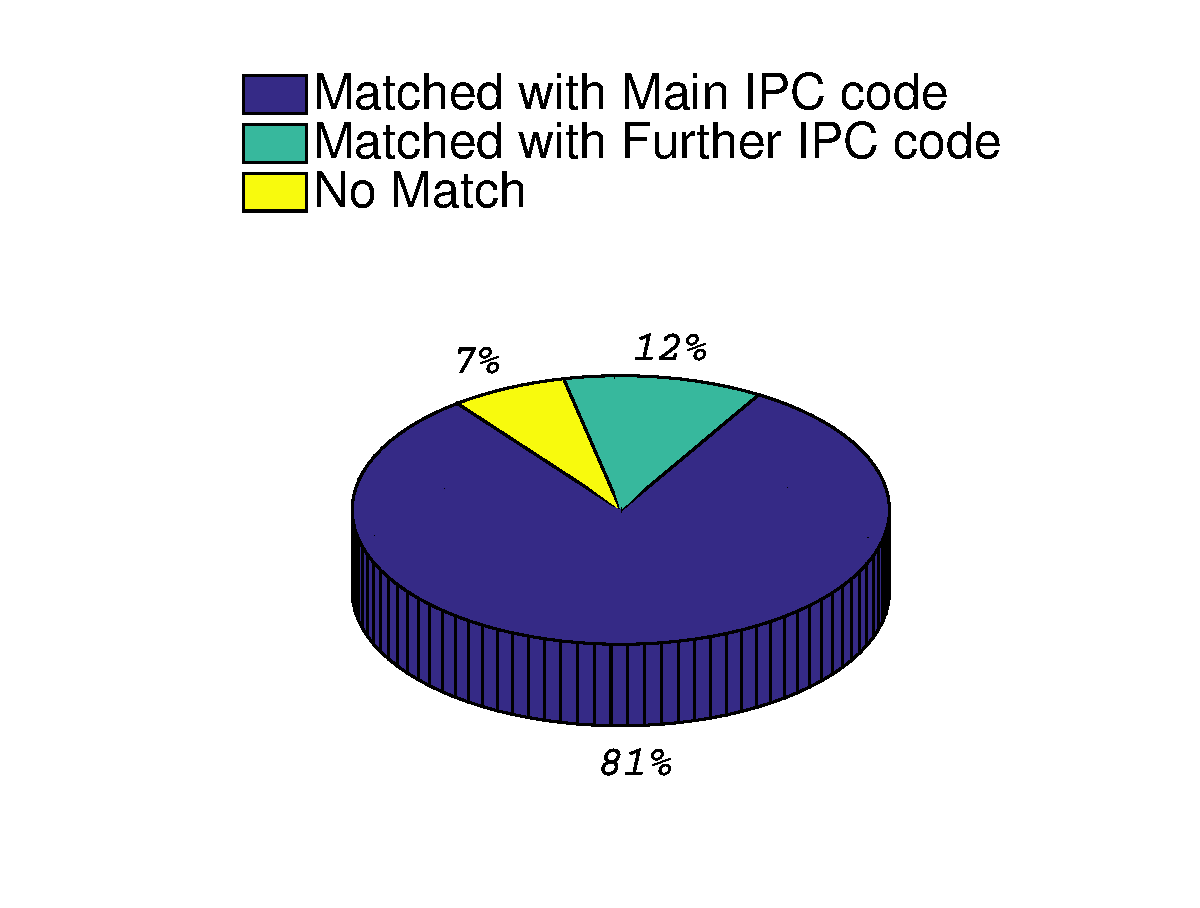
\includegraphics[width=7.5cm, height=6cm]{figs/filter3_pie}} 
\\[1ex]%
\subfigure[The distribution of the number of patents should be processed for each query after applying the IPC filter.
In average, the matching process for each query is done over $ 415,828 $ documents instead of the whole collection (2.6 million documents). This number is much higher than using more restricted filters, so it is not computationally efficient.\label{fig:ipc1stElements_b}]{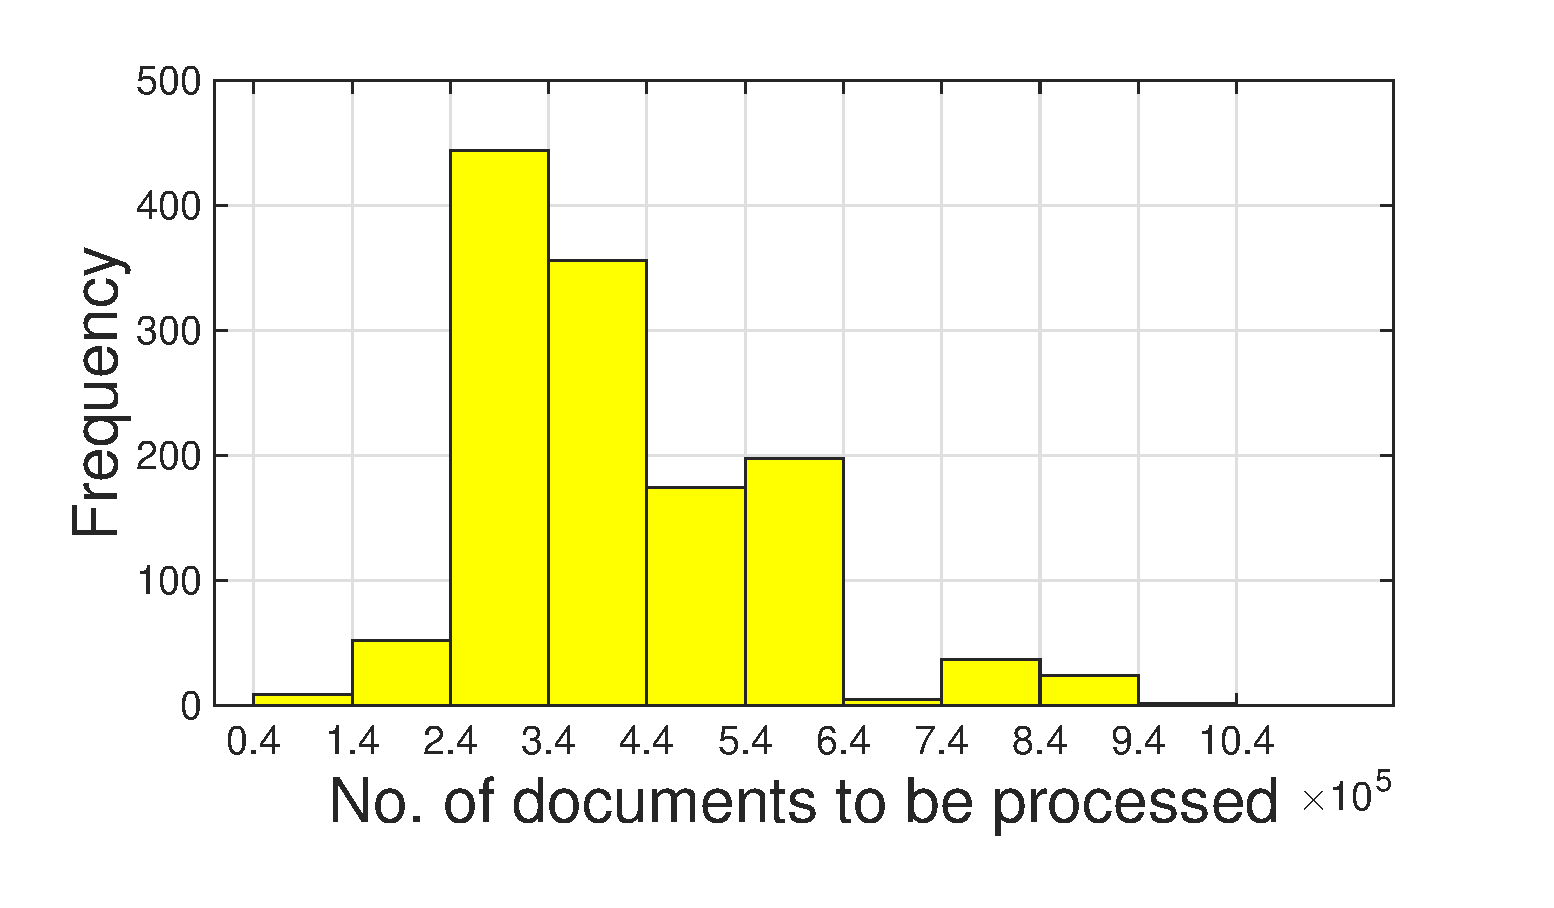
\includegraphics[width=9.5cm , height=6cm]{figs/filter3}} 

\par\end{centering} 
\protect\caption{Applying the first IPC code component for filtering (Section)}
\label{fig:ipc1stElements}
\end{figure}
%%%%%%%%%%%%%%%%%%%%%%%%%%%%%%%%%%%%%%%%%%%%%%%%%%%%%%%%%%%%%%
%%%%%%%%%%%%%%%%%%%%%%%%%%%%%%%%%%%%%%%%%%%%%%%%%%%%%%%%%%%%%%%%%%%%%%%%%%%%%%%%%
%\begin{figure}[t!]
%   \centering
%   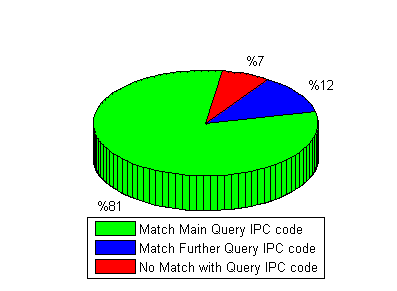
\includegraphics[width=0.50\textwidth,height=55mm]{figs/ipc1stElement.png}
%   \caption{Filter: Only the first component (Section).}   
%   \label{fig:ipc1stElements} 
%\end{figure}
%%%%%%%%%%%%%%%%%%%%%%%%%%%%%%%%%%%%%%%%%%%%%%%%%%%%%%%%%%%%%%%%%%%%%%%%%%%%%%%%%
Figure~\ref{fig:ipc1stElements_a} shows that about 7\% of relevant patents do not share the most general component of the query IPC Code. 
Figure~\ref{fig:ipc1stElements_b} shows the distribution of the number of patents should be ranked for each query after applying the IPC filter.
%: ``\textit{only the first component of the IPC code}". 
The results show that the matching process for each query is done over $ 415,828 $ documents, on average, instead of the whole collection (2.6 million documents). This number is much higher than the number for previous filters, which shows that using only the first component of the IPC code is not computationally efficient because it does not reduce the computational time as well as it still causes 7\% of the errors. 
%The min number of documents considered during matching process is `$ min=41721 $', and the maximum is `$ max=1058447 $'. 
%\vspace{-2em}
%%%%%%%%%%%%%%%%%%%%%%%%%%%%%%%%%%%%%%%%%%%%%%%%%%%%%%%%%%%%%%%%%%%%%%%%%%%%%%%%%
%\begin{figure}[t!]
%   \centering
%   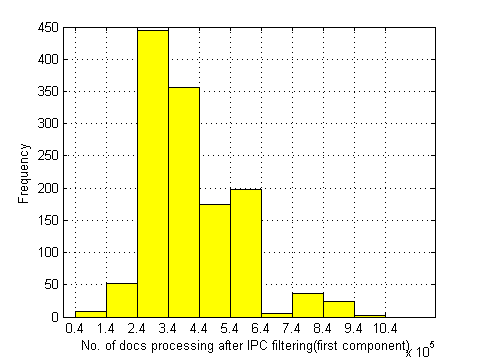
\includegraphics[width=0.60\textwidth,height=60mm]{figs/firstIpcFilter-histo.png}
%   \caption{The distribution of the number of patents should be ranked for a query over all test queries (1303), after applying the IPC filter: ``\textit{only the first component of the IPC code}".
%In average, the matching process for each query is done over `$ 415828 $' documents instead of the whole collection (2.6 million documents). This number is much higher than using more restricted filters and will not be efficient computationally. 
%%The min number of documents considered during matching process is `$ min=41721 $', and the maximum is `$ max=1058447 $'
%}   
%   \label{fig:firstIpcFilter-histo} 
%\end{figure}
%%%%%%%%%%%%%%%%%%%%%%%%%%%%%%%%%%%%%%%%%%%%%%%%%%%%%%%%%%%%%%%%%%%%%%%%%%%%%%%%%

To recap our experiments related to the IPC code filtering, we showed that, in trade off between the errors related to applying IPC code filter and computationally efficient matching process, we got the best results when we applied the first three IPC code (section, class, and subclass) of the reference query as a filter. The filter reduced the number of documents to be ranked from the whole collection to $ 36,254 $ documents on average, so using the IPC filter saved a considerable amount of computational time for us.\\\\